% $Id: board3.tex 9368 2021-08-29 19:28:15Z mskala $

%
% MSK 007 Board 3 build instructions
% Copyright (C) 2017  Matthew Skala
%
% This program is free software: you can redistribute it and/or modify
% it under the terms of the GNU General Public License as published by
% the Free Software Foundation, version 3.
%
% This program is distributed in the hope that it will be useful,
% but WITHOUT ANY WARRANTY; without even the implied warranty of
% MERCHANTABILITY or FITNESS FOR A PARTICULAR PURPOSE.  See the
% GNU General Public License for more details.
%
% You should have received a copy of the GNU General Public License
% along with this program.  If not, see <http://www.gnu.org/licenses/>.
%
% Matthew Skala
% https://northcoastsynthesis.com/
% mskala@northcoastsynthesis.com
%

\chapter{Building Board 3}

The three circuit boards in the Leapfrog Filter are numbered from 1 (closest
to panel) to 3 (furthest from panel), but I recommend building them in the
opposite order, with board 3 first.  One reason is so that if impatient, you
can do the ``pre-adjustment'' (page~\pageref{ch:preadj}) on Board~3 and see
that something is working early in the game, before the other boards are
built.

There are three header connectors on Board~3 which serve to link to Board~2. 
My recommendation is not to solder these in place until you build Board~2,
because it is convenient to assemble the boards into a stack to hold the
connectors in exactly the right places while soldering them.  Accordingly,
the soldering for these connectors is described in that chapter instead of
here.

Note that although I'm describing a separate step for each component value,
and that's how I built mine so as to have plenty of photo opportunities, if
you are reasonably confident about your skills you may find it easier to
populate all or most of the board (i.e.\ put the components in place) and
then solder them in a single step.  Except where noted, the order in which
you add components does not matter much.  I usually describe different
component classes in order of their height from the board (shortest to
tallest) because that usually makes it easier to hold the components to the
board while soldering.

The first PCBs for Board~3 were labelled ``BOARD 3v2'' and had some minor
differences in the silkscreen art, of which the most important was that
R87's value was labelled ``1M.'' That batch was mostly for prototyping, but
there were a few left over which I will sell.  In prototyping I determined
that R87 ought to have the value 390k$\Omega$ instead (to allow a
larger adjustment range for the core DC offset), so if you have a v2 board
you should mount a 390k$\Omega$ resistor in this position regardless of the
silkscreen label.  Later versions (``v3'' and any subsequent) will say
``390k'' here, and I'm putting stickers over the ``1M'' labels on the
existing v2 boards that I sell to help remind DIY builders of the change. 
There is no electrical change in the board itself between v2 and v3; the
updates are all to the silkscreen.

The Board~3 PCB is designed to support modifications.  The resistor network
on this board configures the filter core on Board~2 to produce the desired
response curve, and by substituting other resistor values instead of the
ones shown, you could build a different type of filter (highpass, bandpass,
a different shape of lowpass, or whatever).  A future version of this manual
may include suggested modifications; until then, adventurous
do-it-yourselfers can experiment with calculating their own using the
procedure given starting on page~\pageref{cha:calculations}.  In order to
support alternate curves, there are a few footprints (R28, R29, and R86)
labelled ``OMIT'' on the PCB.  These are not used, and you should just leave
them empty, for the MSK~007's musical near-elliptic low-pass default
response.  Some modified curves might call for mounting components in these
positions.

\section{Preliminaries}

Count out the right number of everything according to the bill of materials. 
There is an abbreviated BOM for Board~3 in Table~\ref{tab:b3bom}, excluding
the headers that will be installed later.

\noindent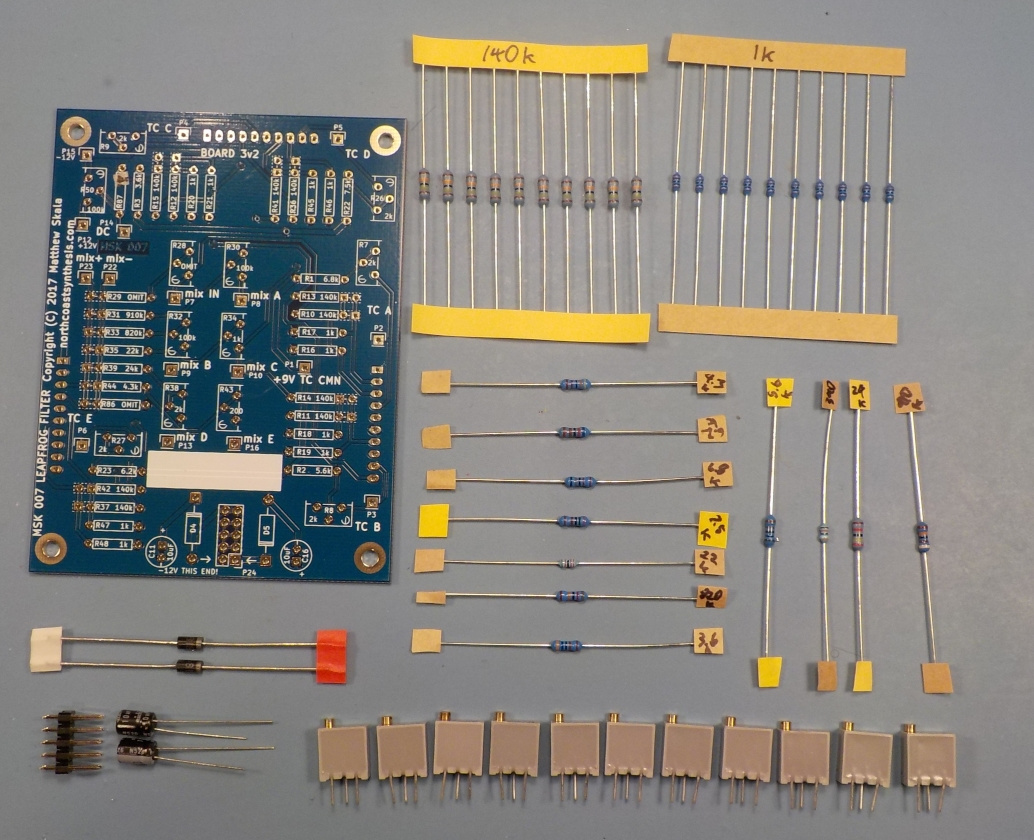
\includegraphics[width=\linewidth]{board3-parts.jpg}

There are 11 multiturn trimmers to be installed on this board.  Before
installing them, use an ohmmeter to adjust each one to 50\% of its range. 
Measure the resistance along the track, then measure the resistance from the
wiper to one end and adjust to make the wiper half the total track
resistance.  This need not be exact, but it will help with adjustment later,
by reducing issues with interaction among the different settings.  With all
trimmers pre-set to 50\%, the module should basically work even if it is not
at its best, whereas if many are installed at extreme values instead, then
you may have trouble getting it up and running enough to adjust it more
accurately.

\begin{table*}
{\centering
\fbox{This table is not a substitute for the text instructions.}
\vspace{\baselineskip}

\begin{tabular}{rp{1in}cp{3in}}
  \textbf{Qty} & \textbf{Ref} & \textbf{Value/Part No.} & \\ \hline
\input{bomdata-3.tex}
\end{tabular}\par}
\caption{Bill of Materials for Board~3.}\label{tab:b3bom}
\end{table*}

\section{Fixed resistors}

In order to allow as many options as possible for modified filter curves
using this same PCB design, many of the resistors on Board~3 have special
three-pin footprints, as shown below.  These are meant to offer the choice
of connecting a signal to the positive or negative input of an op amp or
OTA.

\noindent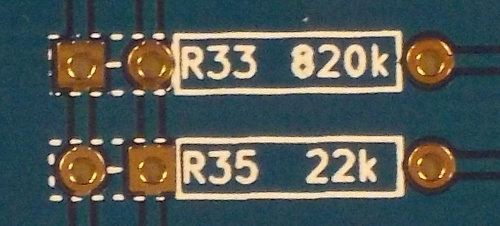
\includegraphics[width=\linewidth]{optres-empty.jpg}

In each of these special footprints the resistor connects between the pad at
right, and \emph{one of} the two pads at left.  The pad you should use for
the default response curve is always the pad with the \emph{square corners},
which may be the nearer or farther pad depending on the individual
footprint.  The other, circular, pad should not be used in a standard build
but is reserved for possible use by some future modification that may
require a different resistor network.

\noindent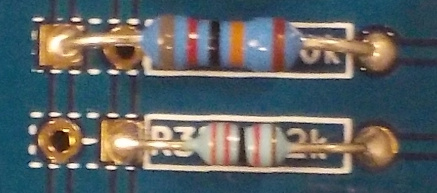
\includegraphics[width=\linewidth]{optres-filled.jpg}

Throughout the installation of the fixed resistors on Board~3, check
carefully against both the pad shapes on the board, and the photos in these
instructions, to be sure you install each resistor into the correct pads. 
Getting any wrong will likely result in little or no response from the
filter, or a highly distorted frequency response curve.

Resistors are never polarized.  I like to install mine in a consistent
direction for cosmetic reasons, but this is electrically unnecessary.  In
this module, metal film 1\%\ resistors are recommended for all fixed-value
resistors.  These will usually have blue bodies and four colour bands
designating the value, plus a fifth band for the tolerance, brown in the
case of 1\%.  These are the resistors normally shipped in the
North Coast kits, but we may occasionally ship better-tolerance resistors (such
as 0.5\%) if we are able to source them at a good price. 
Accordingly, I mention only the four value band colours for this type of
resistor; if you are using resistors with other codes, you are responsible
for knowing them.  Note that colour codes on metal film 1\% resistors are
often ambiguous (reading from one end or the other end may give two
different values, both plausible) and some of the colours are hard to
distinguish anyway.  If in doubt, always measure with an ohmmeter before
soldering the resistor in place.

Install the ten 1k$\Omega$ (brown-black-black-brown) resistors R16 through
R21 and R45 through R48.  These are parts of the voltage dividers
that control input levels for the five integrators making up the filter
core.  A full MSK~007 kit should contain 13 of these resistors, so there
should be three left over for use on the other boards.

\nopagebreak
\noindent\includegraphics[width=\linewidth]{{res-1.0k3}.jpg}

\newpage

Install the 3.6k$\Omega$ (orange-blue-black-brown) resistor R3.  This
resistor controls the linearizing diode current for integrator~C.

\nopagebreak
\noindent\includegraphics[width=\linewidth]{{res-3.6k3}.jpg}

Install the 4.3k$\Omega$ (yellow-orange-black-brown) resistor R44.  This
resistor controls the proportion of integrator~E in the output mix. 
Connect it to the nearer pad.  A full MSK~007 kit should contain two of
these resistors, so there should be one left over for use on Board~2.

\nopagebreak
\noindent\includegraphics[width=\linewidth]{{res-4.3k3}.jpg}

\newpage

Install the 5.6k$\Omega$ (green-blue-black-brown) resistor R2.  This
resistor controls the linearizing diode current for integrator~B.  A full
MSK~007 kit should contain seven of these resistors, so there should be six
left over for use on the other boards.

\nopagebreak
\noindent\includegraphics[width=\linewidth]{{res-5.6k3}.jpg}

Install the 6.2k$\Omega$ (blue-red-black-brown) resistor R23.  This resistor
controls the linearizing diode current for integrator~E.

\nopagebreak
\noindent\includegraphics[width=\linewidth]{{res-6.2k3}.jpg}

\newpage

Install the 6.8k$\Omega$ (blue-grey-black-brown) resistor R1.  This resistor
controls the linearizing diode current for integrator~A.

\nopagebreak
\noindent\includegraphics[width=\linewidth]{{res-6.8k3}.jpg}

Install the 7.5k$\Omega$ (violet-green-black-brown) resistor R22.  This
resistor controls the linearizing diode current for integrator~D.

\nopagebreak
\noindent\includegraphics[width=\linewidth]{{res-7.5k3}.jpg}

\newpage

Install the 22k$\Omega$ (red-red-black-red) resistor R35.  This resistor
controls the proportion of integrator~C in the output mix.  Connect it to
the nearer pad.  A full MSK~007 kit should contain two of these resistors,
so there should be one left over for use on Board~1.

\nopagebreak
\noindent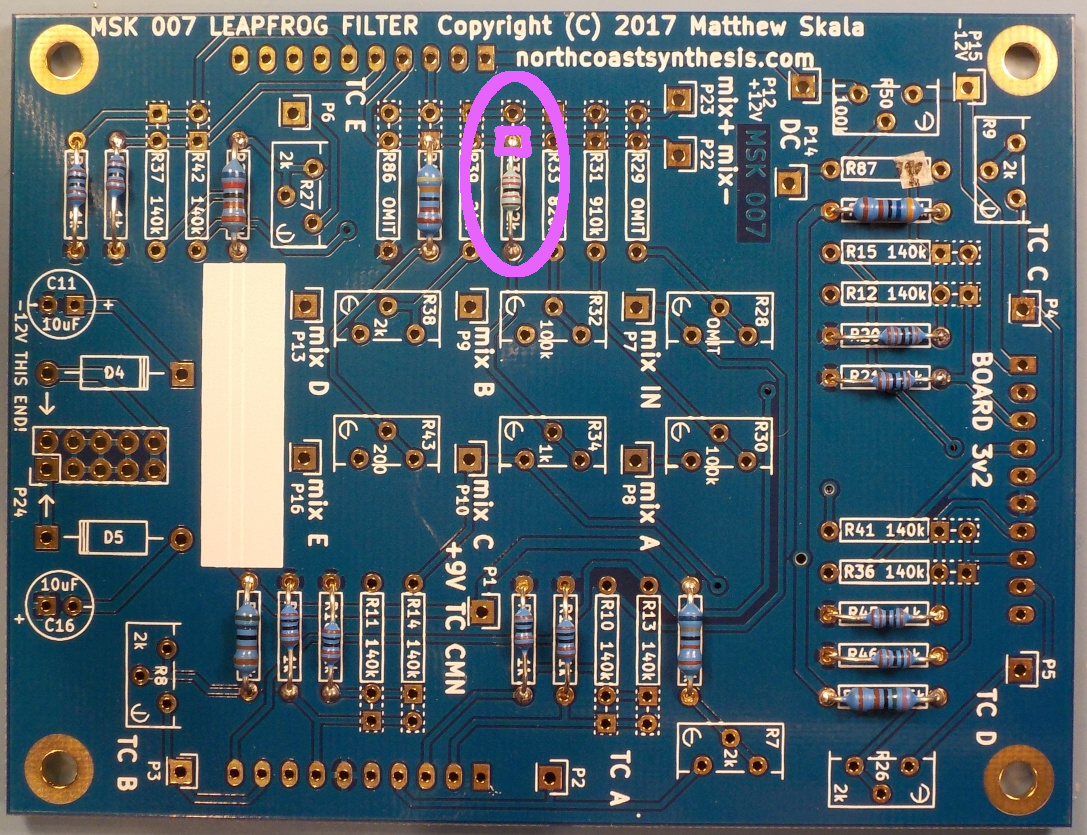
\includegraphics[width=\linewidth]{res-22k3.jpg}

Install the 24k$\Omega$ (red-yellow-black-red) resistor R39.  This resistor
controls the proportion of integrator~D in the output mix.  Connect it to
the farther pad.

\nopagebreak
\noindent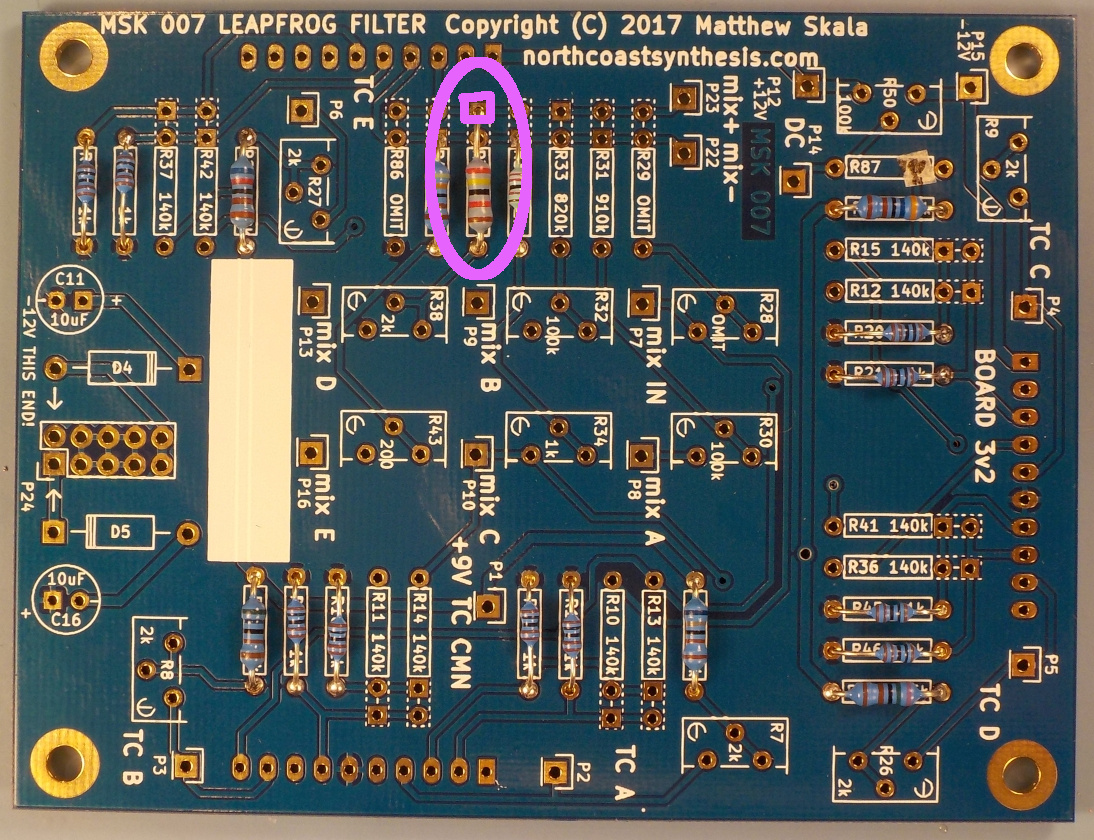
\includegraphics[width=\linewidth]{res-24k3.jpg}

\newpage

Install the ten 140k$\Omega$ (brown-yellow-black-orange) resistors R10
through R15, R36, R37, R41, and R42.  These are parts of the voltage
dividers that control input levels for the five integrators.  The resistors
are installed in five pairs, each with one connected to the nearer and one
connected to the farther pad.  Check the photo and the board pad shapes
carefully.  A full MSK~007 kit should contain 11 of these resistors, leaving
one for use on Board~2.

\nopagebreak
\noindent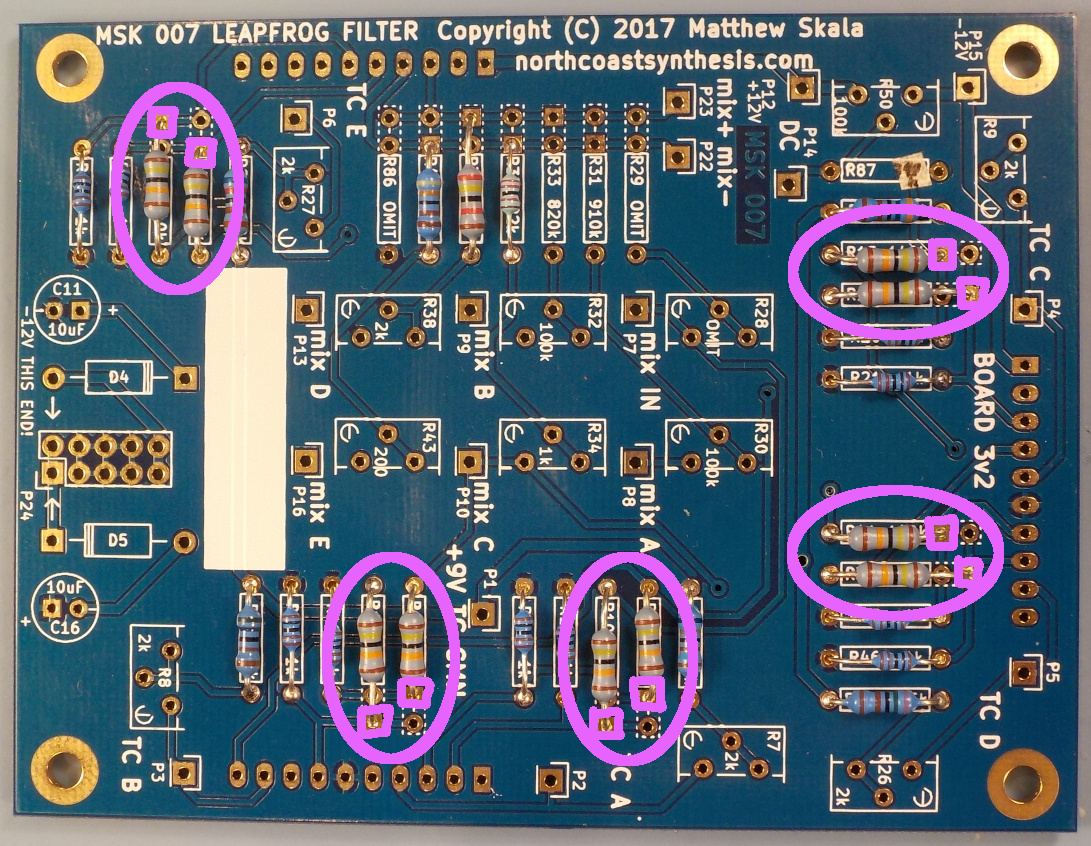
\includegraphics[width=\linewidth]{res-140k3.jpg}

Install the 390k$\Omega$ (orange-white-black-orange) resistor R87.  This
resistor sets the adjustment range for the core DC offset trimmer.  Note that
if you have a v2 board (like the one in the photo) then the silkscreen for
this resistor will read ``1M'' and possibly be covered by a bit of tape;
nonetheless, you should install a 390k$\Omega$ resistor here.

\nopagebreak
\noindent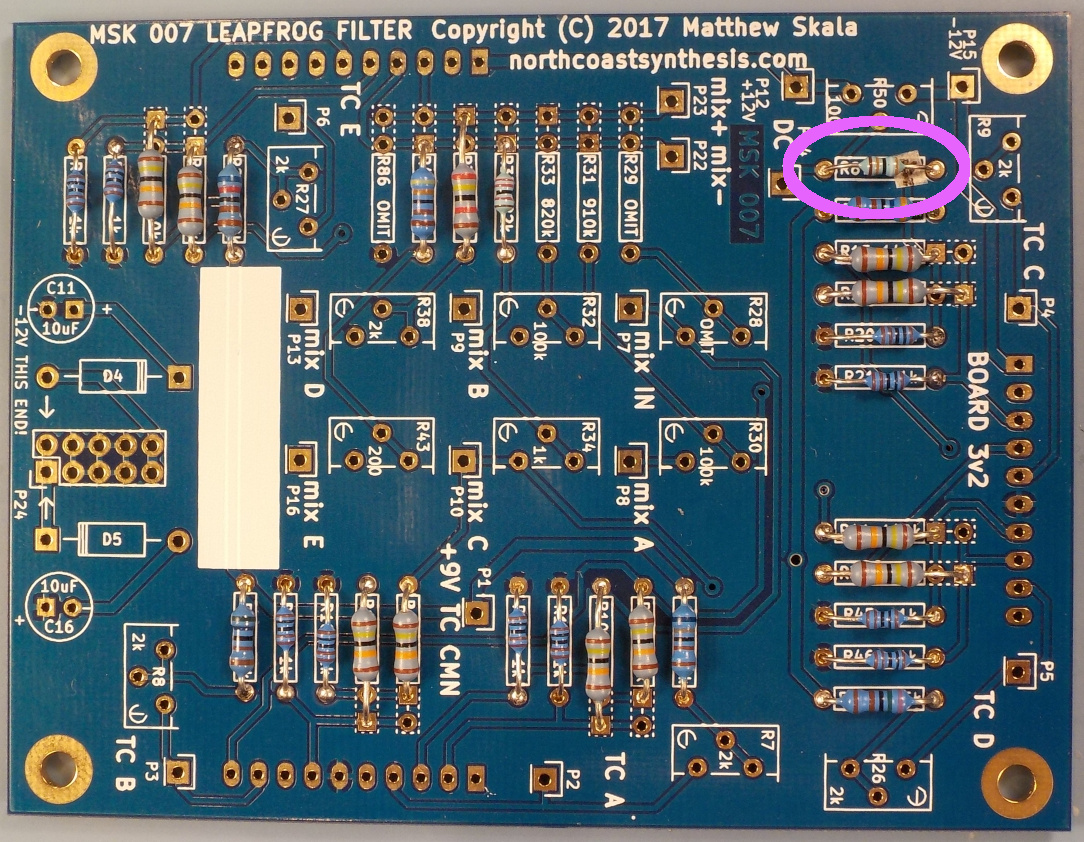
\includegraphics[width=\linewidth]{res-390k3.jpg}

\newpage

Install the 820k$\Omega$ (grey-red-black-orange) resistor R33.  This resistor
controls the proportion of integrator~B in the output mix.  Connect it to
the farther pad.

\nopagebreak
\noindent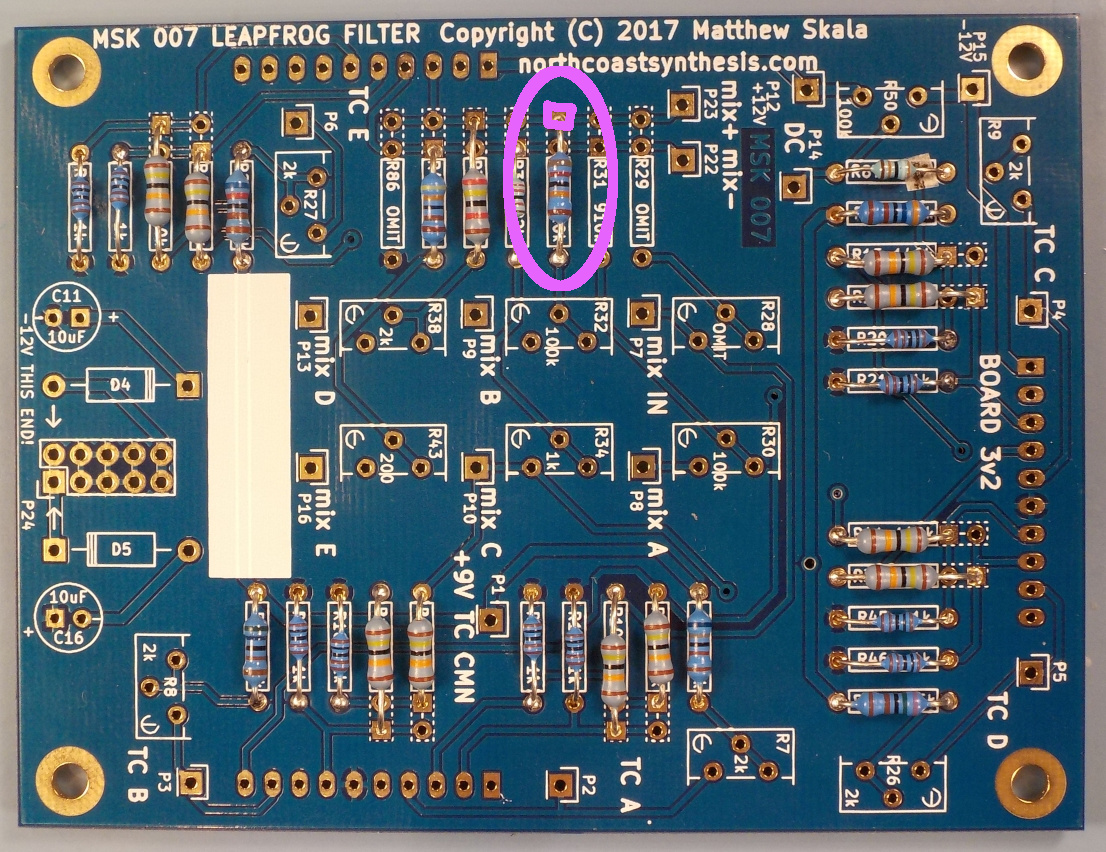
\includegraphics[width=\linewidth]{res-820k3.jpg}

Install the 910k$\Omega$ (white-brown-black-orange) resistor R31.  This
resistor controls the proportion of integrator~A in the output mix.  Connect
it to the nearer pad.

\nopagebreak
\noindent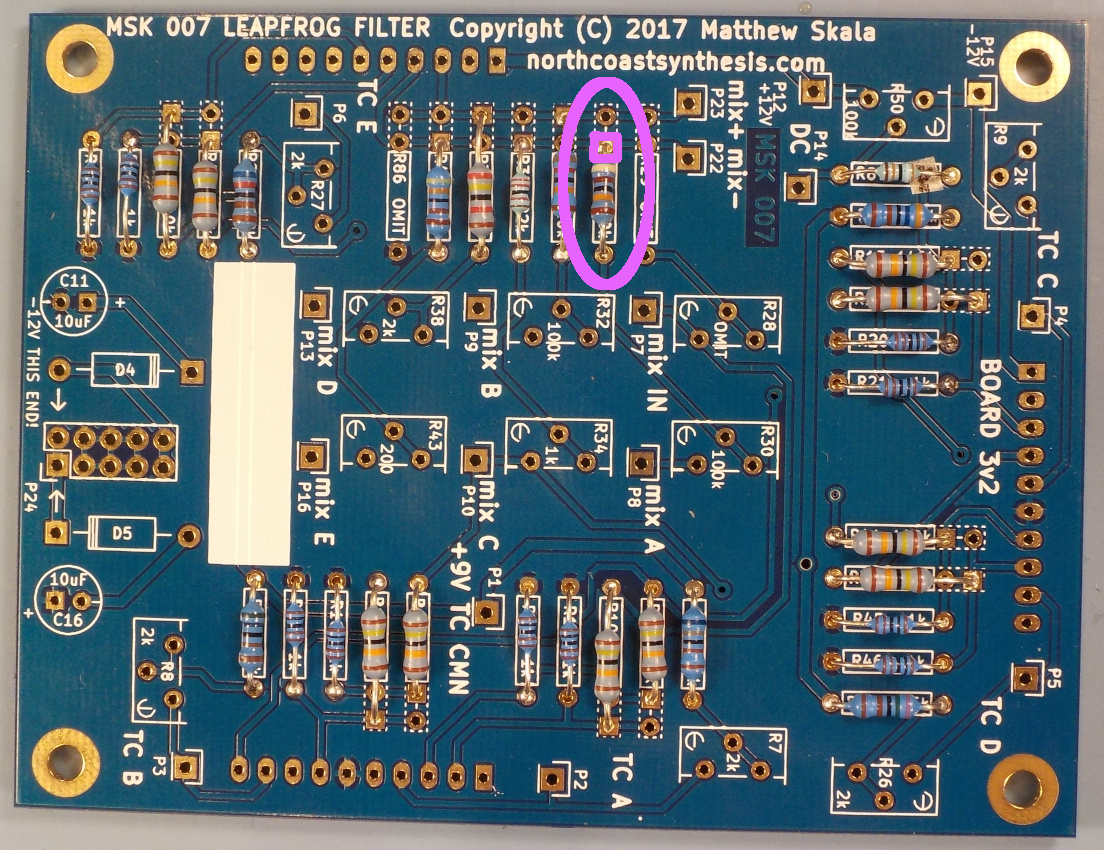
\includegraphics[width=\linewidth]{res-910k3.jpg}

\section{Semiconductors}

Install the two Schottky diodes D4 and D5.  These protect the module against
reverse connection of the power supply.  They are polarized and must be
installed in the correct direction; otherwise they will prevent the module
from operating.  One end of each diode will be marked, usually with a stripe
of grey paint around the black plastic body of the diode.  That end is the
cathode.  The diode outline on the PCB silkscreen is marked with a
similar stripe showing the direction of the cathode, and the solder pad for
the cathode is square instead of round.

\noindent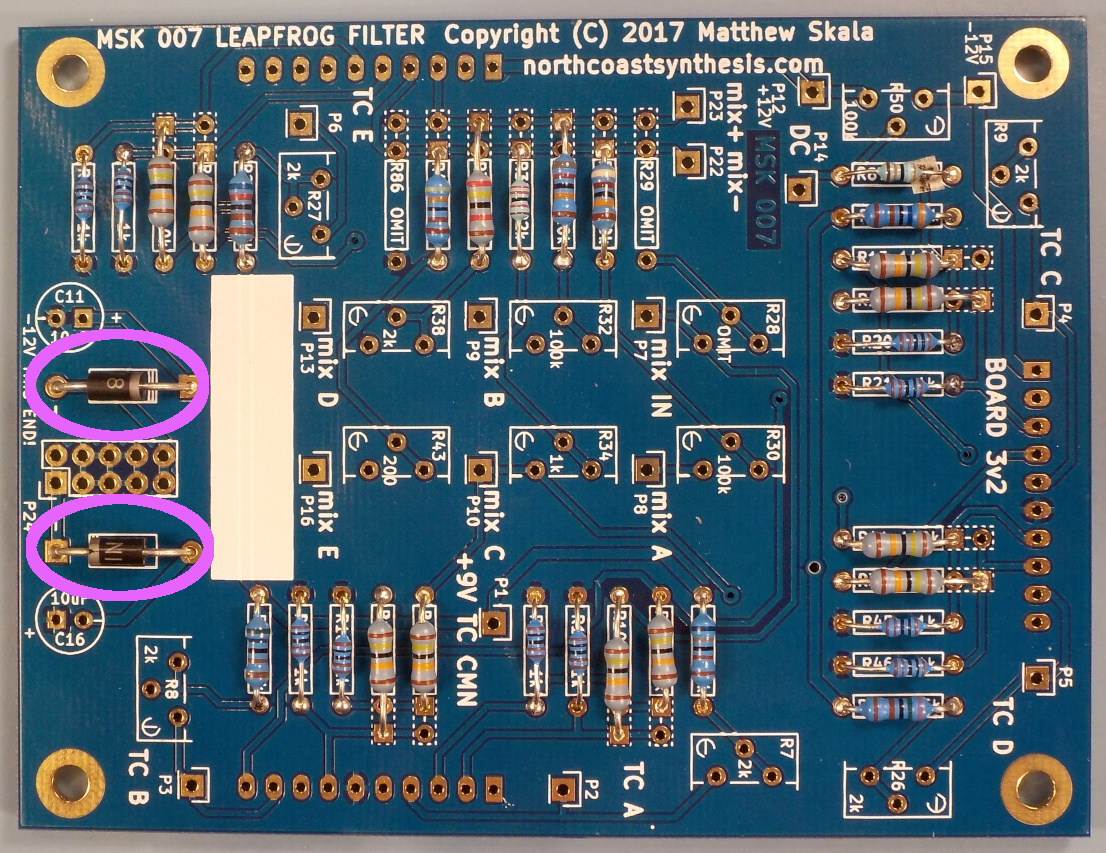
\includegraphics[width=\linewidth]{schottky.jpg}

\section{Electrolytic capacitors}

Install the two 10$\mu$F electrolytic capacitors C11 and C16.  These filter
incoming power to prevent noise in the case power system from affecting the
Leapfrog.  They are polarized components, and may explode if connected
backwards.  As such, there are multiple clues to help you install them in
the right direction.  The negative leg of each capacitor will be marked in
some way, usually with a printed stripe and minus signs on the plastic
wrapping of the capacitor body.  The negative leg of the capacitor will
usually also be shorter, though that is less reliable than the body
markings.  On the PCB, the positive and negative pads are marked with
positive and negative signs in the silkscreen, and the solder pads
themselves are round for negative and square for positive.

\noindent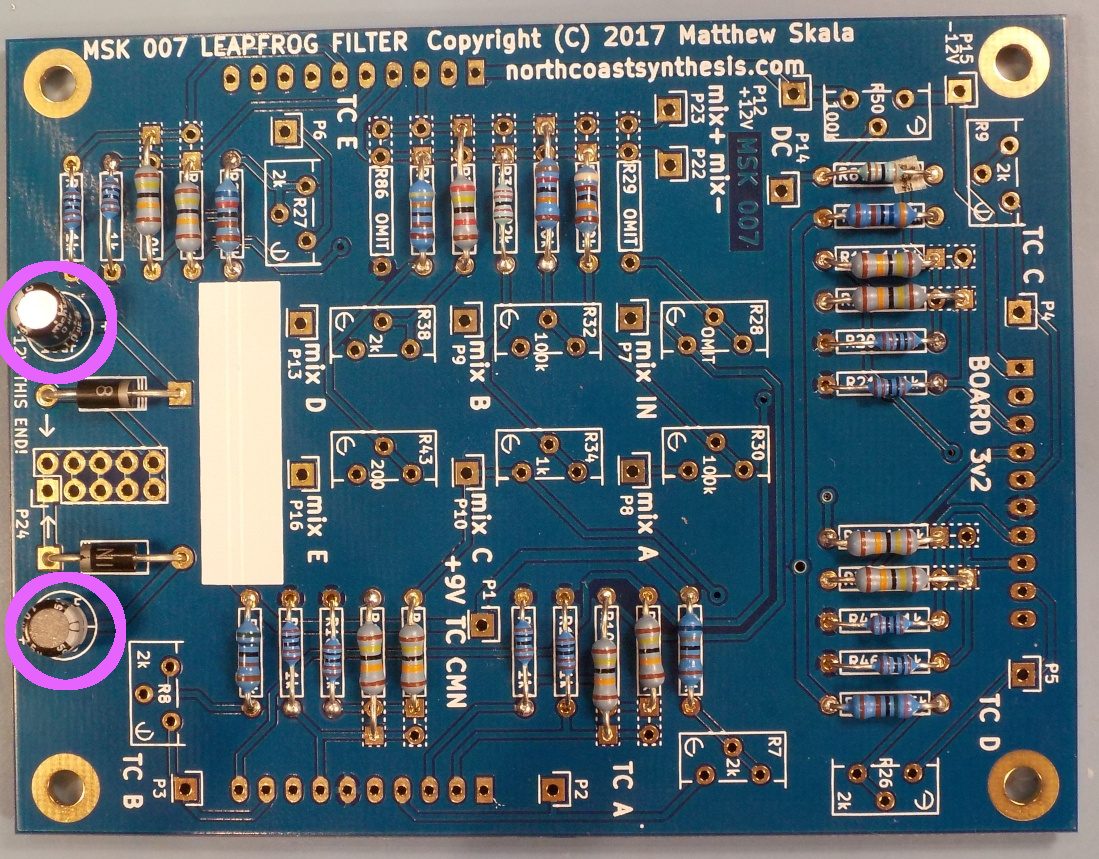
\includegraphics[width=\linewidth]{cap-10u3.jpg}

A full MSK~007 kit should contain four of these capacitors, leaving two
for installation on Board~2.

\section{Trimmer potentiometers}

If you have not already set the trimmers to 50\%\ of their full scale value
as described under ``Preliminaries'' above, then do it now.

Trimmers are not exactly polarized, but the three legs of each trimmer serve
different functions and need to be connected to the right holes.  The
physical arrangement of the legs and corresponding holes should make it
impossible to install the trimmers wrong way round.

Install the 200$\Omega$ trimmer R43.  This trimmer sets the proportion of
integrator~E in the output mix.

\nopagebreak
\noindent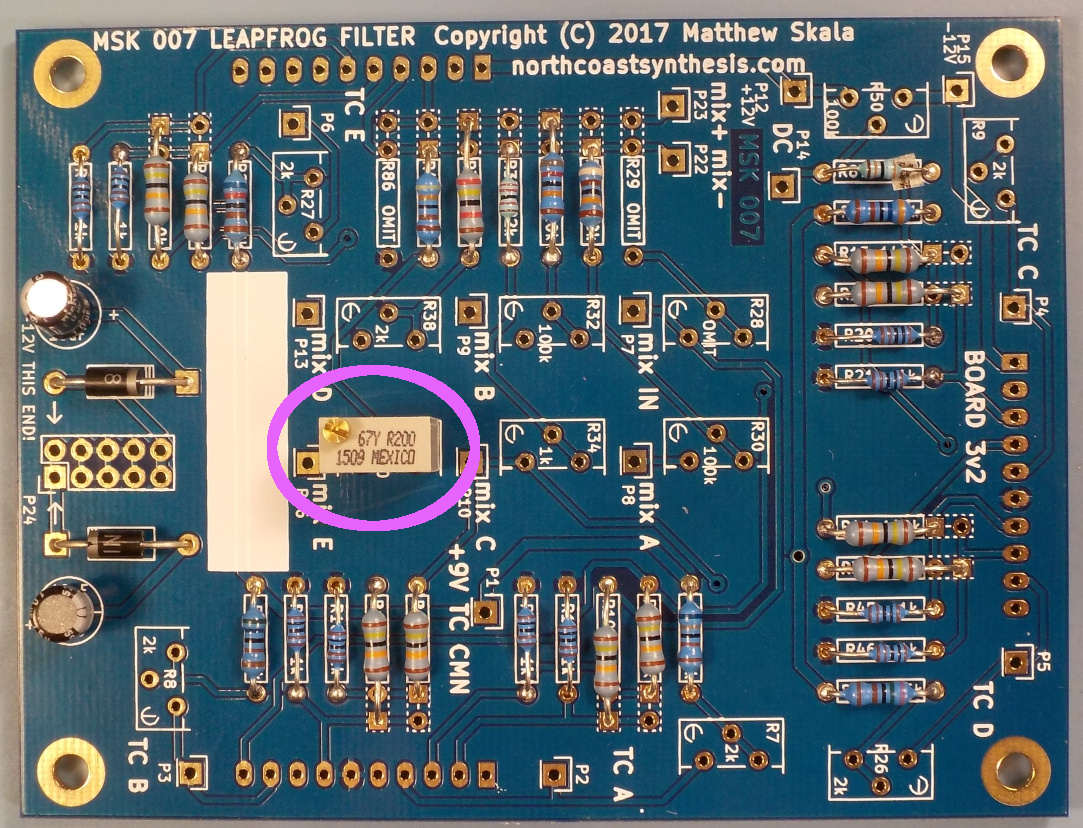
\includegraphics[width=\linewidth]{pot-200w3.jpg}

Install the 1k$\Omega$ trimmer R35.  This trimmer sets the proportion of
integrator~C in the output mix.

\nopagebreak
\noindent\includegraphics[width=\linewidth]{{pot-1.0k3}.jpg}

\newpage

Install the six 2k$\Omega$ trimmers R7 to R9, R26, R27, and R38.  Most of
these are for adjusting the diode currents, and indirectly the time
constants, of the integrator stages; R38 sets the proportion of integrator~D
in the output mix.

\nopagebreak
\noindent\includegraphics[width=\linewidth]{{pot-2.0k3}.jpg}

Install the three 100k$\Omega$ trimmers R30, R32, and R50.  The first two of
these set the output mix amounts for integrators~A and~B respectively; R50
is for adjusting the filter core DC offset.

\nopagebreak
\noindent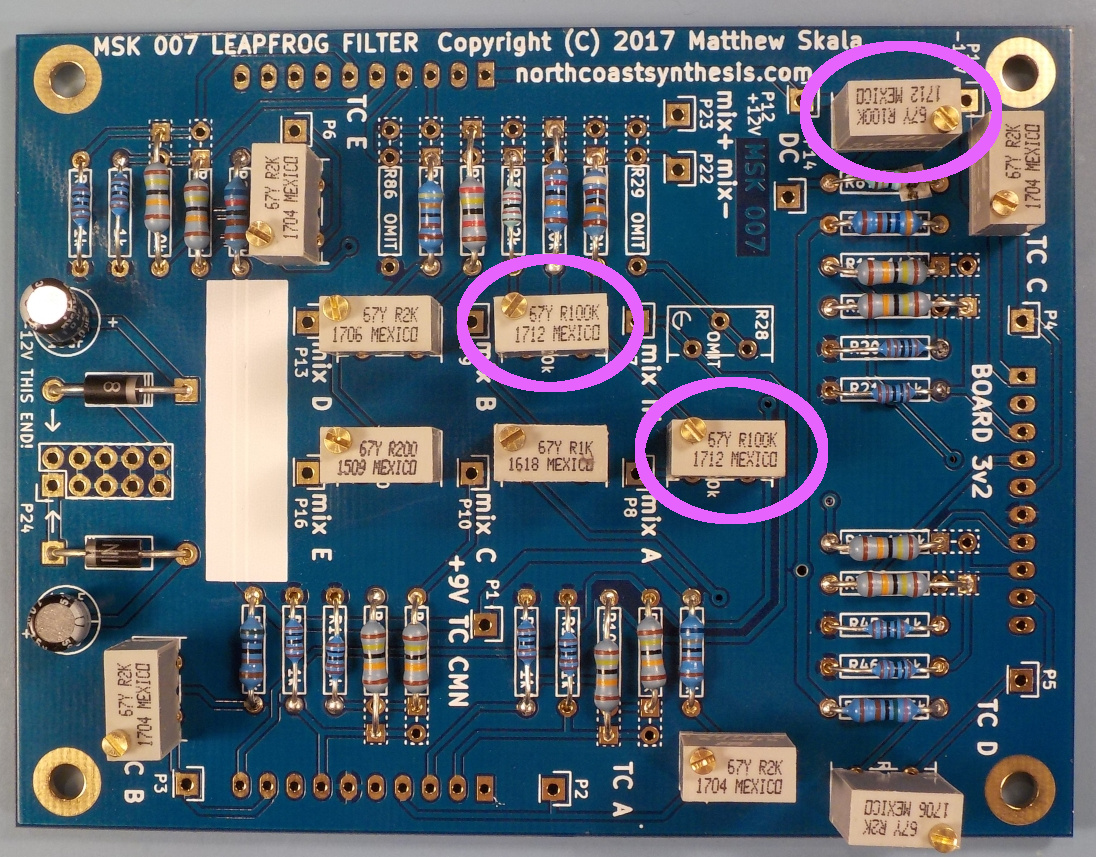
\includegraphics[width=\linewidth]{pot-100k3.jpg}

\section{Power header}

Install the 10-pin dual-row Eurorack power header P24.  It is not polarized
in the horizontal plane.  However, if it has shorter legs on one side, then
those are the ones that should go through the PCB (leaving the longer legs
sticking up to mate with the connector on the power cable), and if it has
tin plating on one end of the pins and gold on the other, then the tin side
should be the one soldered through the board.  Secure the header carefully
to the board, possibly with tape, before soldering it.  It is easy to
accidentally solder it at an angle, which is a difficult error to fix and
may cause trouble when you later attach the power cable.

\noindent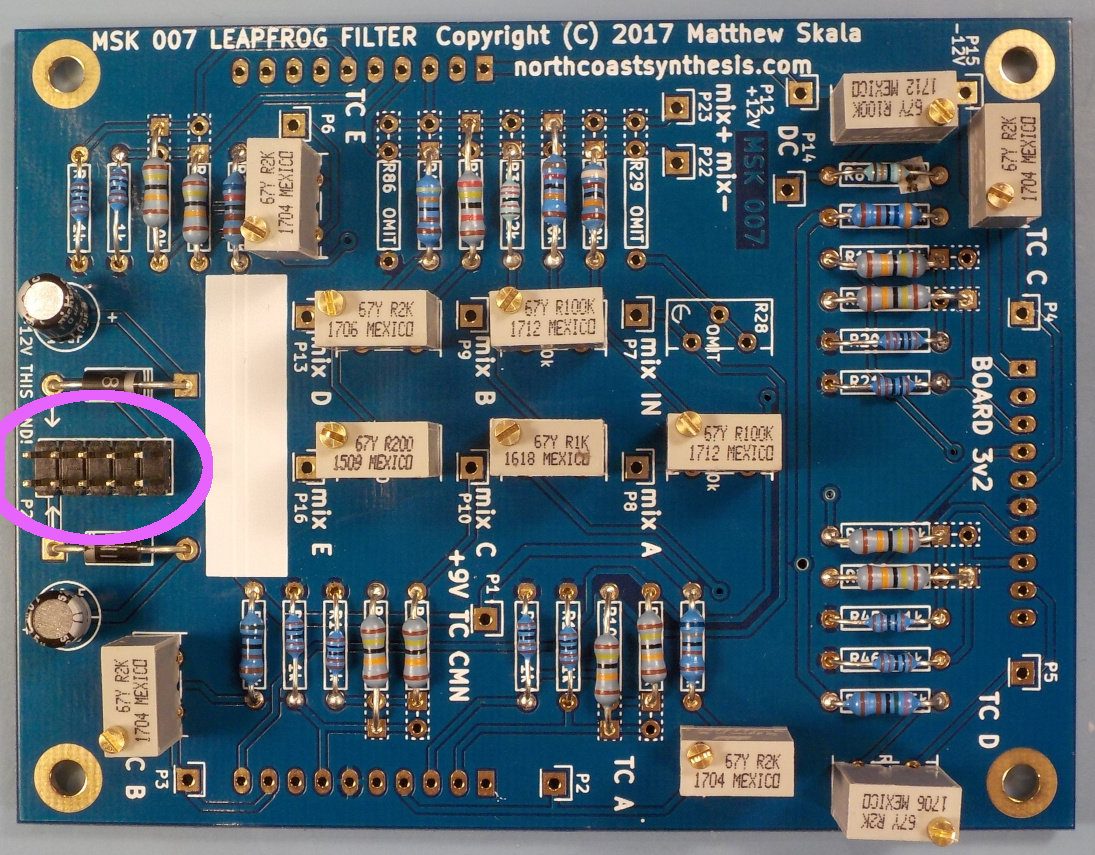
\includegraphics[width=\linewidth]{power.jpg}

Note that Eurorack power connections are polarized even if the connectors
are not.  The cables are usually grey ribbon type with a red stripe along
one side indicating pin 1, which carries $-$12V power.  For most modules
including the MSK~007, the red stripe should be at the \emph{bottom} when
the module is mounted vertically in a case.  On the MSK~007, the correct
location of the $-$12V supply is also marked with the text ``$-$12V THIS
END!'' and arrows on both sides of the PCB silkscreen.  This module is
also protected (by the Schottky diodes you just installed) from damage in
case of a reversed power connection; if you connect the power backwards and
nothing else is wrong, then the module will not power up but will be fine
once you connect the power correctly.  However, many other modules are not
so protected, and it is dangerous to get into the habit of depending on
protection diodes.  Destroying a module by connecting power backwards is
almost a rite of passage for Eurorack users.

At this point you may, if you wish, do the pre-adjustment procedure
described starting on page~\pageref{ch:preadj}.  Whether you do that now or
leave it until the rest of the build is complete, in between completed
boards is a good time to take a break.
